\section{Algoritmo de Floyd-Warshall}

\begin{frame}[fragile]{Algoritmo de Floyd-Warshall}

    \begin{itemize}
        \item Assim como os algoritmos de Bellman-Ford e de Dijkstra, o algoritmo de
            Floyd-Warshall também resolve o problema do caminho mínimo

        \item Ao contrário dos dois citados, ele computa as distâncias mínimos entre todos os
            pares de vértices conectados em uma só execução

        \item O vetor bidimensional que mantém as distância entre todos os pares é inicializado
            com os pesos das arestas entre os nós, e infinito quando não houver uma aresta
            entre os dois vértices

        \item Naturalmente, a distância de um nó a si mesmo é zero

        \item A cada iteração, o algoritmo tenta melhorar as distâncias por meio do uso de
            um vértice intermediário

        \item A complexidade é $O(V^3)$.
    \end{itemize}

\end{frame}

\begin{frame}[fragile]{Visualização do algoritmo de Floyd-Warshall}

    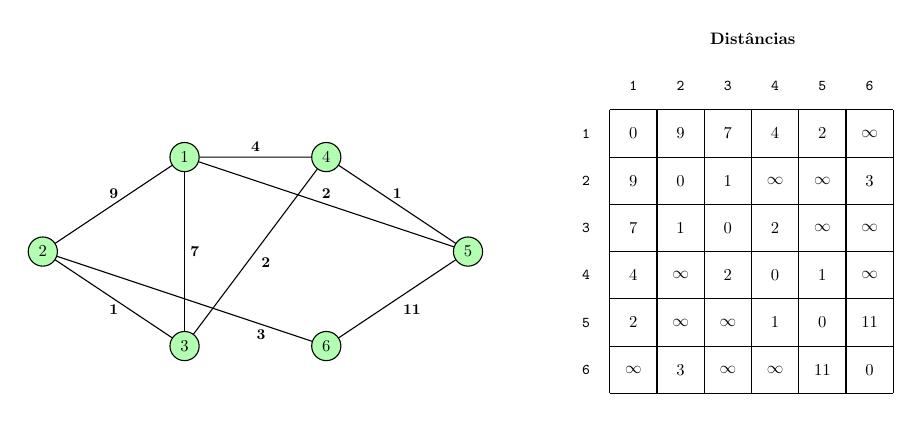
\begin{tikzpicture}[scale=0.6,every node/.style={scale=0.6}]
        \node[anchor=west] at (14, 9.5) { \textbf{Distâncias} };
        \draw (12, 2) grid (18, 8);

        \node at (12.5, 8.5) { \small \texttt{1} };
        \node at (13.5, 8.5) { \small \texttt{2} };
        \node at (14.5, 8.5) { \small \texttt{3} };
        \node at (15.5, 8.5) { \small \texttt{4} };
        \node at (16.5, 8.5) { \small \texttt{5} };
        \node at (17.5, 8.5) { \small \texttt{6} };

        \node at (11.5, 7.5) { \small \texttt{1} };
        \node at (11.5, 6.5) { \small \texttt{2} };
        \node at (11.5, 5.5) { \small \texttt{3} };
        \node at (11.5, 4.5) { \small \texttt{4} };
        \node at (11.5, 3.5) { \small \texttt{5} };
        \node at (11.5, 2.5) { \small \texttt{6} };

        \node at (12.5, 7.5) { $0$ };
        \node at (13.5, 7.5) { $9$ };
        \node at (14.5, 7.5) { $7$ };
        \node at (15.5, 7.5) { $4$ };
        \node at (16.5, 7.5) { $2$ };
        \node at (17.5, 7.5) { $\infty$ };

        \node at (12.5, 6.5) { $9$ };
        \node at (13.5, 6.5) { $0$ };
        \node at (14.5, 6.5) { $1$ };
        \node at (15.5, 6.5) { $\infty$ };
        \node at (16.5, 6.5) { $\infty$ };
        \node at (17.5, 6.5) { $3$ };

        \node at (12.5, 5.5) { $7$ };
        \node at (13.5, 5.5) { $1$ };
        \node at (14.5, 5.5) { $0$ };
        \node at (15.5, 5.5) { $2$ };
        \node at (16.5, 5.5) { $\infty$ };
        \node at (17.5, 5.5) { $\infty$ };

        \node at (12.5, 4.5) { $4$ };
        \node at (13.5, 4.5) { $\infty$ };
        \node at (14.5, 4.5) { $2$ };
        \node at (15.5, 4.5) { $0$ };
        \node at (16.5, 4.5) { $1$ };
        \node at (17.5, 4.5) { $\infty$ };

        \node at (12.5, 3.5) { $2$ };
        \node at (13.5, 3.5) { $\infty$ };
        \node at (14.5, 3.5) { $\infty$ };
        \node at (15.5, 3.5) { $1$ };
        \node at (16.5, 3.5) { $0$ };
        \node at (17.5, 3.5) { $11$ };

        \node at (12.5, 2.5) { $\infty$ };
        \node at (13.5, 2.5) { $3$ };
        \node at (14.5, 2.5) { $\infty$ };
        \node at (15.5, 2.5) { $\infty$ };
        \node at (16.5, 2.5) { $11$ };
        \node at (17.5, 2.5) { $0$ };

        \node[circle, draw, fill=green!30] (a) at (3, 7) {1};
        \node[circle, draw, fill=green!30] (b) at (0, 5) {2};
        \node[circle, draw, fill=green!30] (c) at (3, 3) {3};
        \node[circle, draw, fill=green!30] (d) at (6, 7) {4};
        \node[circle, draw, fill=green!30] (e) at (9, 5) {5};
        \node[circle, draw, fill=green!30] (f) at (6, 3) {6};

        \draw (a) to node[midway,anchor=south] { \small \bfseries 9 } (b);
        \draw (a) to node[midway,anchor=west] { \small \bfseries 7 } (c);
        \draw (a) to node[midway,anchor=south] { \small \bfseries 4 } (d);
        \draw (a) to node[midway,anchor=south] { \small \bfseries 2 } (e);
        \draw (b) to node[midway,anchor=north] { \small \bfseries 1 } (c);
        \draw (b) to node[pos=0.8,anchor=north] { \small \bfseries 3 } (f);
        \draw (c) to node[midway,anchor=north west] { \small \bfseries 2 } (d);
        \draw (d) to node[midway,anchor=south] { \small \bfseries 1 } (e);
        \draw (e) to node[midway,anchor=north west] { \small \bfseries 11 } (f);

    \end{tikzpicture}

\end{frame}

\begin{frame}[fragile]{Visualização do algoritmo de Floyd-Warshall}

    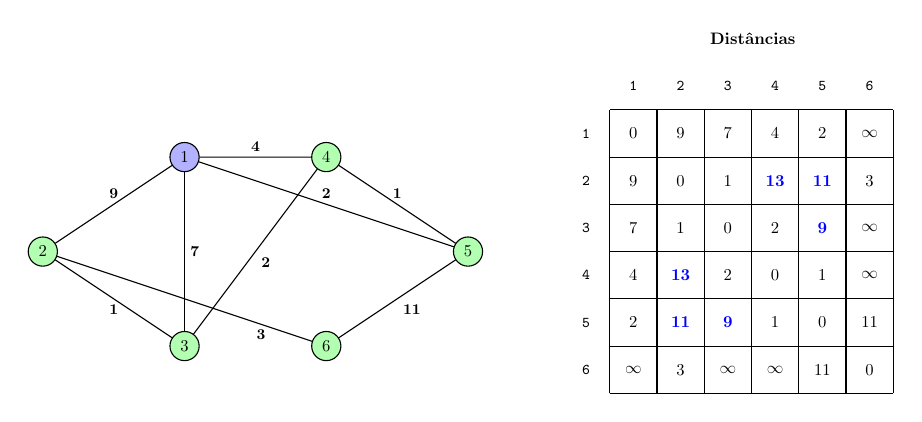
\begin{tikzpicture}[scale=0.6,every node/.style={scale=0.6}]
        \node[anchor=west] at (14, 9.5) { \textbf{Distâncias} };
        \draw (12, 2) grid (18, 8);

        \node at (12.5, 8.5) { \small \texttt{1} };
        \node at (13.5, 8.5) { \small \texttt{2} };
        \node at (14.5, 8.5) { \small \texttt{3} };
        \node at (15.5, 8.5) { \small \texttt{4} };
        \node at (16.5, 8.5) { \small \texttt{5} };
        \node at (17.5, 8.5) { \small \texttt{6} };

        \node at (11.5, 7.5) { \small \texttt{1} };
        \node at (11.5, 6.5) { \small \texttt{2} };
        \node at (11.5, 5.5) { \small \texttt{3} };
        \node at (11.5, 4.5) { \small \texttt{4} };
        \node at (11.5, 3.5) { \small \texttt{5} };
        \node at (11.5, 2.5) { \small \texttt{6} };

        \node at (12.5, 7.5) { $0$ };
        \node at (13.5, 7.5) { $9$ };
        \node at (14.5, 7.5) { $7$ };
        \node at (15.5, 7.5) { $4$ };
        \node at (16.5, 7.5) { $2$ };
        \node at (17.5, 7.5) { $\infty$ };

        \node at (12.5, 6.5) { $9$ };
        \node at (13.5, 6.5) { $0$ };
        \node at (14.5, 6.5) { $1$ };
        \node at (15.5, 6.5) { \textcolor{blue}{$\mathbf{13}$} };
        \node at (16.5, 6.5) { \textcolor{blue}{$\mathbf{11}$} };
        \node at (17.5, 6.5) { $3$ };

        \node at (12.5, 5.5) { $7$ };
        \node at (13.5, 5.5) { $1$ };
        \node at (14.5, 5.5) { $0$ };
        \node at (15.5, 5.5) { $2$ };
        \node at (16.5, 5.5) { \textcolor{blue}{$\mathbf{9}$} };
        \node at (17.5, 5.5) { $\infty$ };

        \node at (12.5, 4.5) { $4$ };
        \node at (13.5, 4.5) { \textcolor{blue}{$\mathbf{13}$} };
        \node at (14.5, 4.5) { $2$ };
        \node at (15.5, 4.5) { $0$ };
        \node at (16.5, 4.5) { $1$ };
        \node at (17.5, 4.5) { $\infty$ };

        \node at (12.5, 3.5) { $2$ };
        \node at (13.5, 3.5) { \textcolor{blue}{$\mathbf{11}$} };
        \node at (14.5, 3.5) { \textcolor{blue}{$\mathbf{9}$} };
        \node at (15.5, 3.5) { $1$ };
        \node at (16.5, 3.5) { $0$ };
        \node at (17.5, 3.5) { $11$ };

        \node at (12.5, 2.5) { $\infty$ };
        \node at (13.5, 2.5) { $3$ };
        \node at (14.5, 2.5) { $\infty$ };
        \node at (15.5, 2.5) { $\infty$ };
        \node at (16.5, 2.5) { $11$ };
        \node at (17.5, 2.5) { $0$ };

        \node[circle, draw, fill=blue!30] (a) at (3, 7) {1};
        \node[circle, draw, fill=green!30] (b) at (0, 5) {2};
        \node[circle, draw, fill=green!30] (c) at (3, 3) {3};
        \node[circle, draw, fill=green!30] (d) at (6, 7) {4};
        \node[circle, draw, fill=green!30] (e) at (9, 5) {5};
        \node[circle, draw, fill=green!30] (f) at (6, 3) {6};

        \draw (a) to node[midway,anchor=south] { \small \bfseries 9 } (b);
        \draw (a) to node[midway,anchor=west] { \small \bfseries 7 } (c);
        \draw (a) to node[midway,anchor=south] { \small \bfseries 4 } (d);
        \draw (a) to node[midway,anchor=south] { \small \bfseries 2 } (e);
        \draw (b) to node[midway,anchor=north] { \small \bfseries 1 } (c);
        \draw (b) to node[pos=0.8,anchor=north] { \small \bfseries 3 } (f);
        \draw (c) to node[midway,anchor=north west] { \small \bfseries 2 } (d);
        \draw (d) to node[midway,anchor=south] { \small \bfseries 1 } (e);
        \draw (e) to node[midway,anchor=north west] { \small \bfseries 11 } (f);

    \end{tikzpicture}

\end{frame}

\begin{frame}[fragile]{Visualização do algoritmo de Floyd-Warshall}

    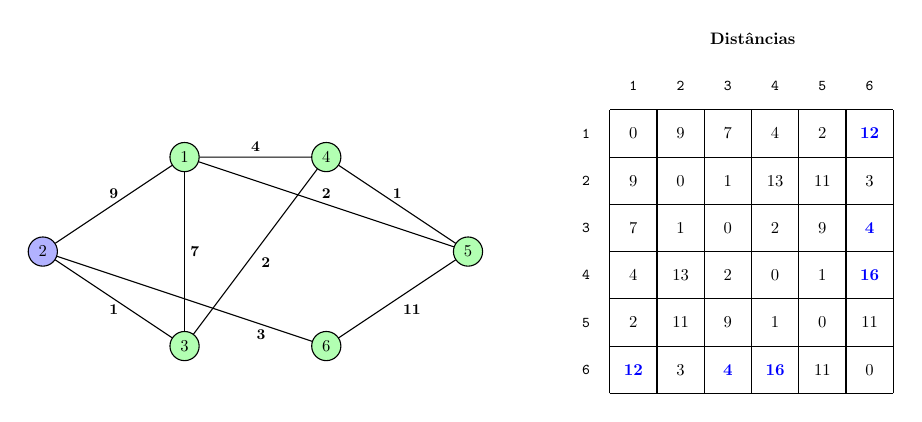
\begin{tikzpicture}[scale=0.6,every node/.style={scale=0.6}]
        \node[anchor=west] at (14, 9.5) { \textbf{Distâncias} };
        \draw (12, 2) grid (18, 8);

        \node at (12.5, 8.5) { \small \texttt{1} };
        \node at (13.5, 8.5) { \small \texttt{2} };
        \node at (14.5, 8.5) { \small \texttt{3} };
        \node at (15.5, 8.5) { \small \texttt{4} };
        \node at (16.5, 8.5) { \small \texttt{5} };
        \node at (17.5, 8.5) { \small \texttt{6} };

        \node at (11.5, 7.5) { \small \texttt{1} };
        \node at (11.5, 6.5) { \small \texttt{2} };
        \node at (11.5, 5.5) { \small \texttt{3} };
        \node at (11.5, 4.5) { \small \texttt{4} };
        \node at (11.5, 3.5) { \small \texttt{5} };
        \node at (11.5, 2.5) { \small \texttt{6} };

        \node at (12.5, 7.5) { $0$ };
        \node at (13.5, 7.5) { $9$ };
        \node at (14.5, 7.5) { $7$ };
        \node at (15.5, 7.5) { $4$ };
        \node at (16.5, 7.5) { $2$ };
        \node at (17.5, 7.5) { \textcolor{blue}{$\mathbf{12}$} };

        \node at (12.5, 6.5) { $9$ };
        \node at (13.5, 6.5) { $0$ };
        \node at (14.5, 6.5) { $1$ };
        \node at (15.5, 6.5) { $13$ };
        \node at (16.5, 6.5) { $11$ };
        \node at (17.5, 6.5) { $3$ };

        \node at (12.5, 5.5) { $7$ };
        \node at (13.5, 5.5) { $1$ };
        \node at (14.5, 5.5) { $0$ };
        \node at (15.5, 5.5) { $2$ };
        \node at (16.5, 5.5) { $9$ };
        \node at (17.5, 5.5) { \textcolor{blue}{$\mathbf{4}$} };

        \node at (12.5, 4.5) { $4$ };
        \node at (13.5, 4.5) { $13$ };
        \node at (14.5, 4.5) { $2$ };
        \node at (15.5, 4.5) { $0$ };
        \node at (16.5, 4.5) { $1$ };
        \node at (17.5, 4.5) { \textcolor{blue}{$\mathbf{16}$} };

        \node at (12.5, 3.5) { $2$ };
        \node at (13.5, 3.5) { $11$ };
        \node at (14.5, 3.5) { $9$ };
        \node at (15.5, 3.5) { $1$ };
        \node at (16.5, 3.5) { $0$ };
        \node at (17.5, 3.5) { $11$ };

        \node at (12.5, 2.5) { \textcolor{blue}{$\mathbf{12}$} };
        \node at (13.5, 2.5) { $3$ };
        \node at (14.5, 2.5) { \textcolor{blue}{$\mathbf{4}$} };
        \node at (15.5, 2.5) { \textcolor{blue}{$\mathbf{16}$} };
        \node at (16.5, 2.5) { $11$ };
        \node at (17.5, 2.5) { $0$ };

        \node[circle, draw, fill=green!30] (a) at (3, 7) {1};
        \node[circle, draw, fill=blue!30] (b) at (0, 5) {2};
        \node[circle, draw, fill=green!30] (c) at (3, 3) {3};
        \node[circle, draw, fill=green!30] (d) at (6, 7) {4};
        \node[circle, draw, fill=green!30] (e) at (9, 5) {5};
        \node[circle, draw, fill=green!30] (f) at (6, 3) {6};

        \draw (a) to node[midway,anchor=south] { \small \bfseries 9 } (b);
        \draw (a) to node[midway,anchor=west] { \small \bfseries 7 } (c);
        \draw (a) to node[midway,anchor=south] { \small \bfseries 4 } (d);
        \draw (a) to node[midway,anchor=south] { \small \bfseries 2 } (e);
        \draw (b) to node[midway,anchor=north] { \small \bfseries 1 } (c);
        \draw (b) to node[pos=0.8,anchor=north] { \small \bfseries 3 } (f);
        \draw (c) to node[midway,anchor=north west] { \small \bfseries 2 } (d);
        \draw (d) to node[midway,anchor=south] { \small \bfseries 1 } (e);
        \draw (e) to node[midway,anchor=north west] { \small \bfseries 11 } (f);

    \end{tikzpicture}

\end{frame}

\begin{frame}[fragile]{Visualização do algoritmo de Floyd-Warshall}

    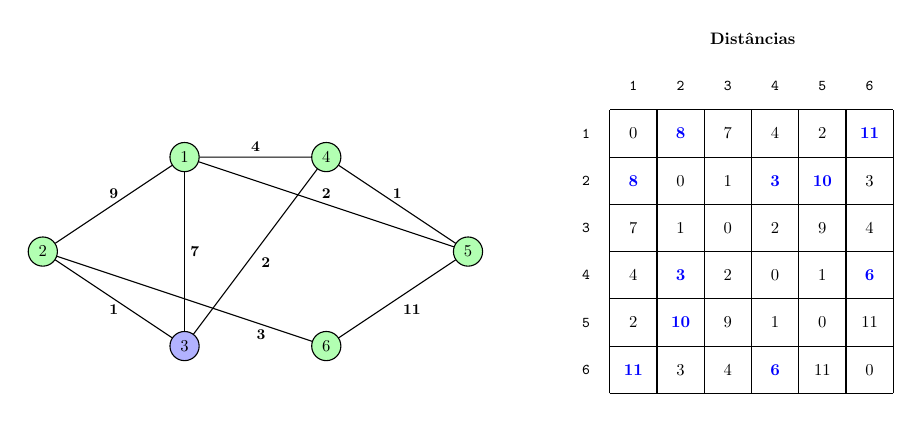
\begin{tikzpicture}[scale=0.6,every node/.style={scale=0.6}]
        \node[anchor=west] at (14, 9.5) { \textbf{Distâncias} };
        \draw (12, 2) grid (18, 8);

        \node at (12.5, 8.5) { \small \texttt{1} };
        \node at (13.5, 8.5) { \small \texttt{2} };
        \node at (14.5, 8.5) { \small \texttt{3} };
        \node at (15.5, 8.5) { \small \texttt{4} };
        \node at (16.5, 8.5) { \small \texttt{5} };
        \node at (17.5, 8.5) { \small \texttt{6} };

        \node at (11.5, 7.5) { \small \texttt{1} };
        \node at (11.5, 6.5) { \small \texttt{2} };
        \node at (11.5, 5.5) { \small \texttt{3} };
        \node at (11.5, 4.5) { \small \texttt{4} };
        \node at (11.5, 3.5) { \small \texttt{5} };
        \node at (11.5, 2.5) { \small \texttt{6} };

        \node at (12.5, 7.5) { $0$ };
        \node at (13.5, 7.5) { \textcolor{blue}{$\mathbf{8}$} };
        \node at (14.5, 7.5) { $7$ };
        \node at (15.5, 7.5) { $4$ };
        \node at (16.5, 7.5) { $2$ };
        \node at (17.5, 7.5) { \textcolor{blue}{$\mathbf{11}$} };

        \node at (12.5, 6.5) { \textcolor{blue}{$\mathbf{8}$} };
        \node at (13.5, 6.5) { $0$ };
        \node at (14.5, 6.5) { $1$ };
        \node at (15.5, 6.5) { \textcolor{blue}{$\mathbf{3}$} };
        \node at (16.5, 6.5) { \textcolor{blue}{$\mathbf{10}$} };
        \node at (17.5, 6.5) { $3$ };

        \node at (12.5, 5.5) { $7$ };
        \node at (13.5, 5.5) { $1$ };
        \node at (14.5, 5.5) { $0$ };
        \node at (15.5, 5.5) { $2$ };
        \node at (16.5, 5.5) { $9$ };
        \node at (17.5, 5.5) { $4$ };

        \node at (12.5, 4.5) { $4$ };
        \node at (13.5, 4.5) { \textcolor{blue}{$\mathbf{3}$} };
        \node at (14.5, 4.5) { $2$ };
        \node at (15.5, 4.5) { $0$ };
        \node at (16.5, 4.5) { $1$ };
        \node at (17.5, 4.5) { \textcolor{blue}{$\mathbf{6}$} };

        \node at (12.5, 3.5) { $2$ };
        \node at (13.5, 3.5) { \textcolor{blue}{$\mathbf{10}$} };
        \node at (14.5, 3.5) { $9$ };
        \node at (15.5, 3.5) { $1$ };
        \node at (16.5, 3.5) { $0$ };
        \node at (17.5, 3.5) { $11$ };

        \node at (12.5, 2.5) { \textcolor{blue}{$\mathbf{11}$} };
        \node at (13.5, 2.5) { $3$ };
        \node at (14.5, 2.5) { $4$ };
        \node at (15.5, 2.5) { \textcolor{blue}{$\mathbf{6}$} };
        \node at (16.5, 2.5) { $11$ };
        \node at (17.5, 2.5) { $0$ };

        \node[circle, draw, fill=green!30] (a) at (3, 7) {1};
        \node[circle, draw, fill=green!30] (b) at (0, 5) {2};
        \node[circle, draw, fill=blue!30] (c) at (3, 3) {3};
        \node[circle, draw, fill=green!30] (d) at (6, 7) {4};
        \node[circle, draw, fill=green!30] (e) at (9, 5) {5};
        \node[circle, draw, fill=green!30] (f) at (6, 3) {6};

        \draw (a) to node[midway,anchor=south] { \small \bfseries 9 } (b);
        \draw (a) to node[midway,anchor=west] { \small \bfseries 7 } (c);
        \draw (a) to node[midway,anchor=south] { \small \bfseries 4 } (d);
        \draw (a) to node[midway,anchor=south] { \small \bfseries 2 } (e);
        \draw (b) to node[midway,anchor=north] { \small \bfseries 1 } (c);
        \draw (b) to node[pos=0.8,anchor=north] { \small \bfseries 3 } (f);
        \draw (c) to node[midway,anchor=north west] { \small \bfseries 2 } (d);
        \draw (d) to node[midway,anchor=south] { \small \bfseries 1 } (e);
        \draw (e) to node[midway,anchor=north west] { \small \bfseries 11 } (f);

    \end{tikzpicture}

\end{frame}

\begin{frame}[fragile]{Visualização do algoritmo de Floyd-Warshall}

    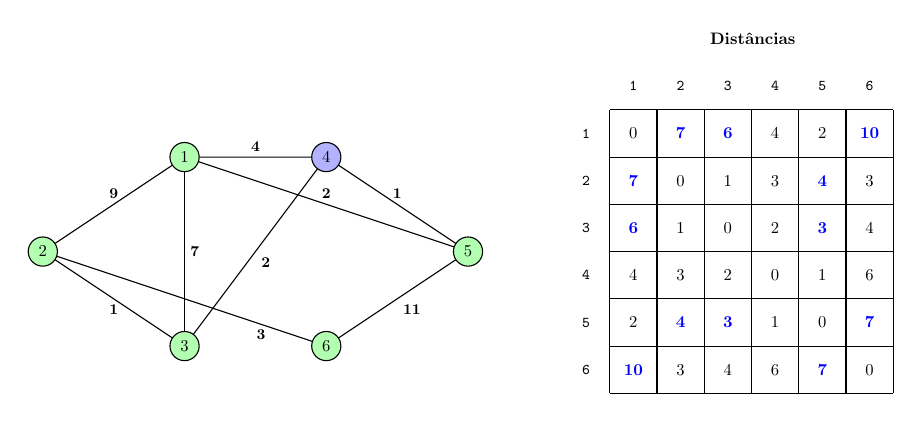
\begin{tikzpicture}[scale=0.6,every node/.style={scale=0.6}]
        \node[anchor=west] at (14, 9.5) { \textbf{Distâncias} };
        \draw (12, 2) grid (18, 8);

        \node at (12.5, 8.5) { \small \texttt{1} };
        \node at (13.5, 8.5) { \small \texttt{2} };
        \node at (14.5, 8.5) { \small \texttt{3} };
        \node at (15.5, 8.5) { \small \texttt{4} };
        \node at (16.5, 8.5) { \small \texttt{5} };
        \node at (17.5, 8.5) { \small \texttt{6} };

        \node at (11.5, 7.5) { \small \texttt{1} };
        \node at (11.5, 6.5) { \small \texttt{2} };
        \node at (11.5, 5.5) { \small \texttt{3} };
        \node at (11.5, 4.5) { \small \texttt{4} };
        \node at (11.5, 3.5) { \small \texttt{5} };
        \node at (11.5, 2.5) { \small \texttt{6} };

        \node at (12.5, 7.5) { $0$ };
        \node at (13.5, 7.5) { \textcolor{blue}{$\mathbf{7}$} };
        \node at (14.5, 7.5) { \textcolor{blue}{$\mathbf{6}$} };
        \node at (15.5, 7.5) { $4$ };
        \node at (16.5, 7.5) { $2$ };
        \node at (17.5, 7.5) { \textcolor{blue}{$\mathbf{10}$} };

        \node at (12.5, 6.5) { \textcolor{blue}{$\mathbf{7}$} };
        \node at (13.5, 6.5) { $0$ };
        \node at (14.5, 6.5) { $1$ };
        \node at (15.5, 6.5) { $3$ };
        \node at (16.5, 6.5) { \textcolor{blue}{$\mathbf{4}$} };
        \node at (17.5, 6.5) { $3$ };

        \node at (12.5, 5.5) { \textcolor{blue}{$\mathbf{6}$} };
        \node at (13.5, 5.5) { $1$ };
        \node at (14.5, 5.5) { $0$ };
        \node at (15.5, 5.5) { $2$ };
        \node at (16.5, 5.5) { \textcolor{blue}{$\mathbf{3}$} };
        \node at (17.5, 5.5) { $4$ };

        \node at (12.5, 4.5) { $4$ };
        \node at (13.5, 4.5) { $3$ };
        \node at (14.5, 4.5) { $2$ };
        \node at (15.5, 4.5) { $0$ };
        \node at (16.5, 4.5) { $1$ };
        \node at (17.5, 4.5) { $6$ };

        \node at (12.5, 3.5) { $2$ };
        \node at (13.5, 3.5) { \textcolor{blue}{$\mathbf{4}$} };
        \node at (14.5, 3.5) { \textcolor{blue}{$\mathbf{3}$} };
        \node at (15.5, 3.5) { $1$ };
        \node at (16.5, 3.5) { $0$ };
        \node at (17.5, 3.5) { \textcolor{blue}{$\mathbf{7}$} };

        \node at (12.5, 2.5) { \textcolor{blue}{$\mathbf{10}$} };
        \node at (13.5, 2.5) { $3$ };
        \node at (14.5, 2.5) { $4$ };
        \node at (15.5, 2.5) { $6$ };
        \node at (16.5, 2.5) { \textcolor{blue}{$\mathbf{7}$} };
        \node at (17.5, 2.5) { $0$ };

        \node[circle, draw, fill=green!30] (a) at (3, 7) {1};
        \node[circle, draw, fill=green!30] (b) at (0, 5) {2};
        \node[circle, draw, fill=green!30] (c) at (3, 3) {3};
        \node[circle, draw, fill=blue!30] (d) at (6, 7) {4};
        \node[circle, draw, fill=green!30] (e) at (9, 5) {5};
        \node[circle, draw, fill=green!30] (f) at (6, 3) {6};

        \draw (a) to node[midway,anchor=south] { \small \bfseries 9 } (b);
        \draw (a) to node[midway,anchor=west] { \small \bfseries 7 } (c);
        \draw (a) to node[midway,anchor=south] { \small \bfseries 4 } (d);
        \draw (a) to node[midway,anchor=south] { \small \bfseries 2 } (e);
        \draw (b) to node[midway,anchor=north] { \small \bfseries 1 } (c);
        \draw (b) to node[pos=0.8,anchor=north] { \small \bfseries 3 } (f);
        \draw (c) to node[midway,anchor=north west] { \small \bfseries 2 } (d);
        \draw (d) to node[midway,anchor=south] { \small \bfseries 1 } (e);
        \draw (e) to node[midway,anchor=north west] { \small \bfseries 11 } (f);

    \end{tikzpicture}

\end{frame}

\begin{frame}[fragile]{Visualização do algoritmo de Floyd-Warshall}

    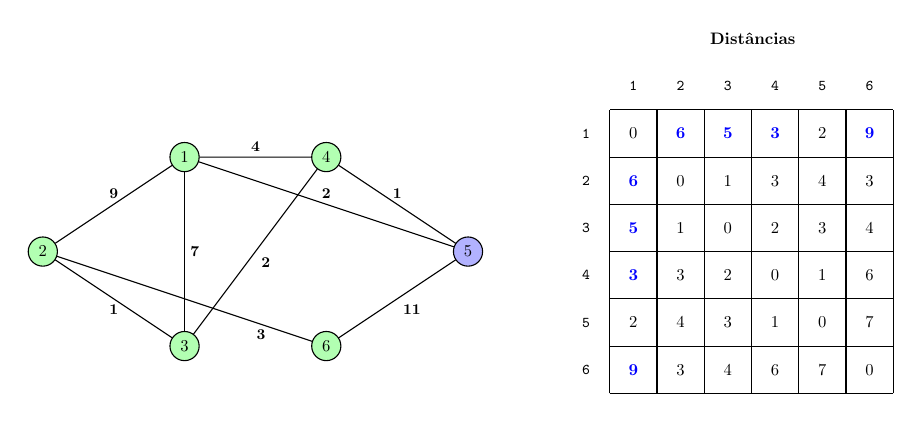
\begin{tikzpicture}[scale=0.6,every node/.style={scale=0.6}]
        \node[anchor=west] at (14, 9.5) { \textbf{Distâncias} };
        \draw (12, 2) grid (18, 8);

        \node at (12.5, 8.5) { \small \texttt{1} };
        \node at (13.5, 8.5) { \small \texttt{2} };
        \node at (14.5, 8.5) { \small \texttt{3} };
        \node at (15.5, 8.5) { \small \texttt{4} };
        \node at (16.5, 8.5) { \small \texttt{5} };
        \node at (17.5, 8.5) { \small \texttt{6} };

        \node at (11.5, 7.5) { \small \texttt{1} };
        \node at (11.5, 6.5) { \small \texttt{2} };
        \node at (11.5, 5.5) { \small \texttt{3} };
        \node at (11.5, 4.5) { \small \texttt{4} };
        \node at (11.5, 3.5) { \small \texttt{5} };
        \node at (11.5, 2.5) { \small \texttt{6} };

        \node at (12.5, 7.5) { $0$ };
        \node at (13.5, 7.5) { \textcolor{blue}{$\mathbf{6}$} };
        \node at (14.5, 7.5) { \textcolor{blue}{$\mathbf{5}$} };
        \node at (15.5, 7.5) { \textcolor{blue}{$\mathbf{3}$} };
        \node at (16.5, 7.5) { $2$ };
        \node at (17.5, 7.5) { \textcolor{blue}{$\mathbf{9}$} };

        \node at (12.5, 6.5) { \textcolor{blue}{$\mathbf{6}$} };
        \node at (13.5, 6.5) { $0$ };
        \node at (14.5, 6.5) { $1$ };
        \node at (15.5, 6.5) { $3$ };
        \node at (16.5, 6.5) { $4$ };
        \node at (17.5, 6.5) { $3$ };

        \node at (12.5, 5.5) { \textcolor{blue}{$\mathbf{5}$} };
        \node at (13.5, 5.5) { $1$ };
        \node at (14.5, 5.5) { $0$ };
        \node at (15.5, 5.5) { $2$ };
        \node at (16.5, 5.5) { $3$ };
        \node at (17.5, 5.5) { $4$ };

        \node at (12.5, 4.5) { \textcolor{blue}{$\mathbf{3}$} };
        \node at (13.5, 4.5) { $3$ };
        \node at (14.5, 4.5) { $2$ };
        \node at (15.5, 4.5) { $0$ };
        \node at (16.5, 4.5) { $1$ };
        \node at (17.5, 4.5) { $6$ };

        \node at (12.5, 3.5) { $2$ };
        \node at (13.5, 3.5) { $4$ };
        \node at (14.5, 3.5) { $3$ };
        \node at (15.5, 3.5) { $1$ };
        \node at (16.5, 3.5) { $0$ };
        \node at (17.5, 3.5) { $7$ };

        \node at (12.5, 2.5) { \textcolor{blue}{$\mathbf{9}$} };
        \node at (13.5, 2.5) { $3$ };
        \node at (14.5, 2.5) { $4$ };
        \node at (15.5, 2.5) { $6$ };
        \node at (16.5, 2.5) { $7$ };
        \node at (17.5, 2.5) { $0$ };

        \node[circle, draw, fill=green!30] (a) at (3, 7) {1};
        \node[circle, draw, fill=green!30] (b) at (0, 5) {2};
        \node[circle, draw, fill=green!30] (c) at (3, 3) {3};
        \node[circle, draw, fill=green!30] (d) at (6, 7) {4};
        \node[circle, draw, fill=blue!30] (e) at (9, 5) {5};
        \node[circle, draw, fill=green!30] (f) at (6, 3) {6};

        \draw (a) to node[midway,anchor=south] { \small \bfseries 9 } (b);
        \draw (a) to node[midway,anchor=west] { \small \bfseries 7 } (c);
        \draw (a) to node[midway,anchor=south] { \small \bfseries 4 } (d);
        \draw (a) to node[midway,anchor=south] { \small \bfseries 2 } (e);
        \draw (b) to node[midway,anchor=north] { \small \bfseries 1 } (c);
        \draw (b) to node[pos=0.8,anchor=north] { \small \bfseries 3 } (f);
        \draw (c) to node[midway,anchor=north west] { \small \bfseries 2 } (d);
        \draw (d) to node[midway,anchor=south] { \small \bfseries 1 } (e);
        \draw (e) to node[midway,anchor=north west] { \small \bfseries 11 } (f);

    \end{tikzpicture}

\end{frame}

\begin{frame}[fragile]{Visualização do algoritmo de Floyd-Warshall}

    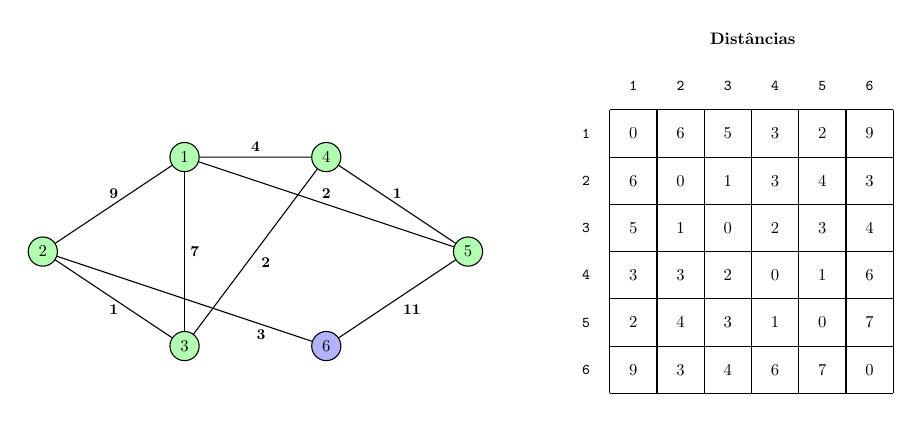
\begin{tikzpicture}[scale=0.6,every node/.style={scale=0.6}]
        \node[anchor=west] at (14, 9.5) { \textbf{Distâncias} };
        \draw (12, 2) grid (18, 8);

        \node at (12.5, 8.5) { \small \texttt{1} };
        \node at (13.5, 8.5) { \small \texttt{2} };
        \node at (14.5, 8.5) { \small \texttt{3} };
        \node at (15.5, 8.5) { \small \texttt{4} };
        \node at (16.5, 8.5) { \small \texttt{5} };
        \node at (17.5, 8.5) { \small \texttt{6} };

        \node at (11.5, 7.5) { \small \texttt{1} };
        \node at (11.5, 6.5) { \small \texttt{2} };
        \node at (11.5, 5.5) { \small \texttt{3} };
        \node at (11.5, 4.5) { \small \texttt{4} };
        \node at (11.5, 3.5) { \small \texttt{5} };
        \node at (11.5, 2.5) { \small \texttt{6} };

        \node at (12.5, 7.5) { $0$ };
        \node at (13.5, 7.5) { $6$ };
        \node at (14.5, 7.5) { $5$ };
        \node at (15.5, 7.5) { $3$ };
        \node at (16.5, 7.5) { $2$ };
        \node at (17.5, 7.5) { $9$ };

        \node at (12.5, 6.5) { $6$ };
        \node at (13.5, 6.5) { $0$ };
        \node at (14.5, 6.5) { $1$ };
        \node at (15.5, 6.5) { $3$ };
        \node at (16.5, 6.5) { $4$ };
        \node at (17.5, 6.5) { $3$ };

        \node at (12.5, 5.5) { $5$ };
        \node at (13.5, 5.5) { $1$ };
        \node at (14.5, 5.5) { $0$ };
        \node at (15.5, 5.5) { $2$ };
        \node at (16.5, 5.5) { $3$ };
        \node at (17.5, 5.5) { $4$ };

        \node at (12.5, 4.5) { $3$ };
        \node at (13.5, 4.5) { $3$ };
        \node at (14.5, 4.5) { $2$ };
        \node at (15.5, 4.5) { $0$ };
        \node at (16.5, 4.5) { $1$ };
        \node at (17.5, 4.5) { $6$ };

        \node at (12.5, 3.5) { $2$ };
        \node at (13.5, 3.5) { $4$ };
        \node at (14.5, 3.5) { $3$ };
        \node at (15.5, 3.5) { $1$ };
        \node at (16.5, 3.5) { $0$ };
        \node at (17.5, 3.5) { $7$ };

        \node at (12.5, 2.5) { $9$ };
        \node at (13.5, 2.5) { $3$ };
        \node at (14.5, 2.5) { $4$ };
        \node at (15.5, 2.5) { $6$ };
        \node at (16.5, 2.5) { $7$ };
        \node at (17.5, 2.5) { $0$ };

        \node[circle, draw, fill=green!30] (a) at (3, 7) {1};
        \node[circle, draw, fill=green!30] (b) at (0, 5) {2};
        \node[circle, draw, fill=green!30] (c) at (3, 3) {3};
        \node[circle, draw, fill=green!30] (d) at (6, 7) {4};
        \node[circle, draw, fill=green!30] (e) at (9, 5) {5};
        \node[circle, draw, fill=blue!30] (f) at (6, 3) {6};

        \draw (a) to node[midway,anchor=south] { \small \bfseries 9 } (b);
        \draw (a) to node[midway,anchor=west] { \small \bfseries 7 } (c);
        \draw (a) to node[midway,anchor=south] { \small \bfseries 4 } (d);
        \draw (a) to node[midway,anchor=south] { \small \bfseries 2 } (e);
        \draw (b) to node[midway,anchor=north] { \small \bfseries 1 } (c);
        \draw (b) to node[pos=0.8,anchor=north] { \small \bfseries 3 } (f);
        \draw (c) to node[midway,anchor=north west] { \small \bfseries 2 } (d);
        \draw (d) to node[midway,anchor=south] { \small \bfseries 1 } (e);
        \draw (e) to node[midway,anchor=north west] { \small \bfseries 11 } (f);

    \end{tikzpicture}

\end{frame}

\begin{frame}[fragile]{Implementação do algoritmo de Floyd-Warshall em C++}
    \inputsnippet{c++}{1}{21}{floyd.cpp}
\end{frame}

\begin{frame}[fragile]{Implementação do algoritmo de Floyd-Warshall em C++}
    \inputsnippet{c++}{22}{42}{floyd.cpp}
\end{frame}

\begin{frame}[fragile]{Identificação do caminho mínimo}

    \begin{itemize}
        \item Assim como nos algoritmos de Bellman-Ford e Dijkstra, é possível recuperar a 
            sequência de arestas que compõem o caminho mínimo

        \item Para determinar o caminho, é preciso manter o vetor bidimensional \code{c++}{pred}, 
            onde \code{c++}{pred[u][v]} é o nó que antecede $v$ no caminho mínimo que vai de $u$ a 
            $v$

        \item Inicialmente, todos os elementos deste vetor devem ser iguais a um valor sentinela,
            exceto em dois casos:

            \begin{enumerate}
                \item \code{c++}{pred[u][u] = u}
                \item \code{c++}{pred[u][v] = u}, se $(u, v)\in E$
            \end{enumerate}

        \item Se o vértice $k$ reduzir a distância \code{c}{dist[u][v]} (isto é, se
            \code{c}{dist[u][k] + dist[k][v] < dist[u][v]}), então o 
            \code{c++}{pred[u][v] = pred[k][v]}

        \item Deste modo, o caminho mínimo de $u$ a $v$ pode ser recuperado, passando por todos os 
            predecessores até se atingir o nó $u$
    \end{itemize}

\end{frame}

\begin{frame}[fragile]{Recuperação do caminho mínimo}
    \inputsnippet{c++}{1}{21}{floyd2.cpp}
\end{frame}

\begin{frame}[fragile]{Recuperação do caminho mínimo}
    \inputsnippet{c++}{23}{43}{floyd2.cpp}
\end{frame}

\begin{frame}[fragile]{Recuperação do caminho mínimo}
    \inputsnippet{c++}{44}{64}{floyd2.cpp}
\end{frame}

\begin{frame}[fragile]{Recuperação do caminho mínimo}
    \inputsnippet{c++}{65}{85}{floyd2.cpp}
\end{frame}
















